%!TeX root =  ../../thesis.tex

\section{Výzvy v IoT}
Vývoj zařízení v rámci Internetů věcí sebou přináší spoustu výzev, jak v rámci designu hardwaru, tak správného a efektivního využití limitovaných prostředků při návrhu softwaru. 

\subsection{Hardwarové}
Hardwarové výzvy jsou především ovlivněny potřebnou velikostí, kdy se na malý deskový počítač musí všechny komponenty a IO pro komunikaci s dalšími zařízeními jako jsou například senzory a ovladače na motorky. Na návrhu hardwaru IoT zařízení je nejtišší navrhnout “tělo” zařízení, kdy například pro dron je důležitá výdrž baterky, ale i jeho samotná váha, což znamená použít lehké, však dostatečně pevný materiál. Je potřeba brát v potaz mnoho atributů zařízení, kdy navýšením jednoho můžeme snížit druhý, například větší baterka znamená delší výdrž, ale také větší váhu.

\subsection{Softwarové}
Při návrhu softwaru pro mikrokontroléry je potřeba dobře zvážit datové typy, jednak aby nedocházelo k přetečení a pak aby se neplýtvalo pamětí, které je podstatně výrazně méně než na moderních počítačích. Pro maximální efektivitu se člověk nevyhne nutné znalosti programovacího jazyka C, jelikož právě skrze C máme největší kontrolu nad hardwarovými prostředky (Assembler neberu v potaz, jelikož se dnes běžně nepoužívá). Při návrhu softwaru pro mikrokontroléry je nejlepší se vyhnout dynamickému alokování paměti, jelikož by nám tímto způsobem mohla rychle dojít, nejlepší je použít buffery, hlavně při práci s textovými řetězci. S těmi se pracuje v takzvaném C-stylu, neboli jako s polem znaků, jelikož C++ textový řetězec std::string je objekt a zabere podstatně více paměti než samotné pole znaků. Sám sem se potýkal s problémy při vývoji softwaru pro tester, kdy mi přetékal buffer na textový řetězec nebo nastal zmatek při práci s odkazem na buffer a ten byl přemazán a výpis na displej nebyl správný.

\subsubsection{Debuggování}
Debugovat mikrokontrolér není tak lehké jako program pro počítač, ale není to nemožné a má-li zařízení možnost komunikace s počítačem, jako například v případě Arduina, můžeme využít sériovou komunikaci skrze USB kabel, kterým do něj nahráváme kód. Jinak se dá využít klasické debuggování pomocí takzvaného krokování.
\begin{figure}[H]
	\centering
	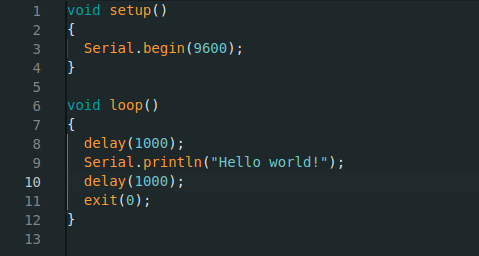
\includegraphics[width=0.9\textwidth]{pictures/code.png}
    	\caption{Ukázka kódu kdy Arduino posálá zprávu do IDE}
   	\label{fig:usbIDE}
\end{figure}

Na obrázku \ref{fig:usbIDE} je kód, který demonstruje jak se dá poslat text do IDE. V setupu je potřeba nastavit modulační rychlost, kdy 9600 je maximum pro Arduino. V metodě loop je pak samotný výstup, kdy sekundové čekání je moc, ale měl by se text vypisovat opakovaně, tak bude potřeba, jinak ho nebudeme stíhat číst.

\begin{figure}[H]
	\centering
	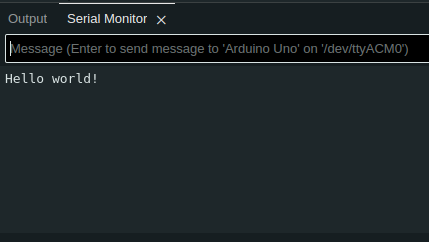
\includegraphics[width=0.9\textwidth]{pictures/message.png}
    	\caption{Ukázka výpisu zprávy z arduina}
   	\label{fig:msgIDE}
\end{figure}
Na obrázku \ref{fig:msgIDE} vidíme konzoli, která je ve spodní části IDE a je v ní text “Hello world!” z ukázky na obrázku \ref{fig:usbIDE}.

